\documentclass{beamer}


\setbeamerfont{footnote}{size=\tiny}
%\AtBeginSection[]
%{
%  \begin{frame}<beamer>
%%    \frametitle{Outline for Section \thesection}
%    \frametitle{Outline}
%    \tableofcontents[currentsection]
%  \end{frame}
%}

\newcommand{\OutlineRedux}
{
  \begin{frame}<beamer>
%    \frametitle{Outline for Section \thesection}
    \frametitle{Outline}
    \tableofcontents[currentsection]
  \end{frame}
}

\usepackage{bbm}
\usepackage{algorithm}
\usepackage{algpseudocodex}
\usepackage{caption}
\usepackage{tikz}
\usetikzlibrary{positioning, arrows.meta}
\usepackage{hyperref}
\hypersetup{colorlinks=true, linkcolor=black, urlcolor=blue, citecolor=red}

\usetheme{CambridgeUS}
\setbeamercolor{title}{bg=red!65!black,fg=white}

\setbeamertemplate{sidebar right}
{
  \vfill%
  \llap{\insertlogo\hskip0.1cm}%
  \vskip2pt%
  \llap{\href{http://domdisanto.github.io}{Downloadable Slides}\hskip0.2cm}% NEW
  \vskip3pt% NEW
  \llap{\usebeamertemplate***{navigation symbols}\hskip0.1cm}%
  \vskip2pt%
}



% Bibliography Options 
\usepackage[url=false, doi=false, maxcitenames=1, isbn=false]{biblatex}
\addbibresource{GNN_Presentation.bib}

\title{Graphical Neural Networks}
%\subtitle{}
\author{Dominic DiSanto}
\institute[]{Department of Biostatistics, Harvard University}
\date{\today}


% Custom commands 
\newcommand{\nhood}{\mathcal{N}}
\newcommand{\Graph}{\mathcal{G}}
\newcommand{\NodeSet}{V}
\newcommand{\NumNodes}{N}
\newcommand{\node}{v}
\newcommand{\nrepresent}{h}
\newcommand{\NodeRepMat}{\mathbf{H}}
\newcommand{\EdgeSet}{E}
\newcommand{\edge}{e}
\newcommand{\DegMat}{\mathbf{D}}
\newcommand{\iter}{\kappa}
\newcommand{\Iter}{K}
\newcommand{\AdjMat}{\mathbf{A}}
\newcommand{\LapMat}{\mathbf{L}}
\newcommand{\LapMatNorm}{\widetilde{\mathbf{L}}}
\newcommand{\ReLu}{\text{ReLu}}
\newcommand{\Ind}{\mathbbm{1}}
\newcommand{\Identity}{\mathbf{I}}

%%%%%%%%%%%%%%%%%%%%%%%%
    % START %%%%%%%%%%%%
%%%%%%%%%%%%%%%%%%%%%%%%
\begin{document}

\begin{frame}[allowframebreaks]{Notes/Questions (To Be Deleted)}
    \begin{itemize}
        \item Touch on geometric DL in general? Or just focus on GNN's and not worry about placing within the DL landscape? 
        \item Touch on AlphaFold? GNN's used I believe but unconfirmed, and architecture is complicated/seems infeasible (at least for my time right now)
        \item Still unsure how to tie in PrimeKG paper
        \item Node-level seems intuitive, my pseudocode already outlines iterative updating of node features and we mention reg/class/multiclass
        \item Methods for edge selection/identification? Some instances we only want to preserve structure, but sometimes we want to predict/fit edges, how does that fit into message-passing/GCN methods or other extensions? 
        \item Example of graph-level classification?  
        \item \textcolor{red}{Diffpool article as extension of general GNN, hierarchical pooling over global readout functions?} \url{https://papers.nips.cc/paper_files/paper/2018/file/e77dbaf6759253c7c6d0efc5690369c7-Paper.pdf}
    \end{itemize}
\end{frame}


\begin{frame}
\maketitle
\end{frame}

\begin{frame}{Outline}
\tableofcontents 
\end{frame}


\section{Set-Up and Motivation \textcolor{red}{5ish minutes}}

\begin{frame}{Goals}
    \begin{itemize}\setlength\itemsep{8mm}
        \item Provide a useful overview of Graphical Neural Networks (GNN)
        \begin{itemize}
            \item Motivation for necessity of GNN's 
            \item Provide a general framework of fitting 
        \end{itemize}
        \item Describe applications and extensions of the general GNN model 
        \begin{itemize}
            \item Multimodal Physiological/Biomedical Data
            \item Integration of Knowledge-Graph and EHR Data
        \end{itemize}
    \end{itemize}
\end{frame}


\begin{frame}{KG Application}
    \textcolor{red}{Image here}
\end{frame}

\begin{frame}{Multi-modal Biomedical Data}
    \begin{figure}
        \centering 
        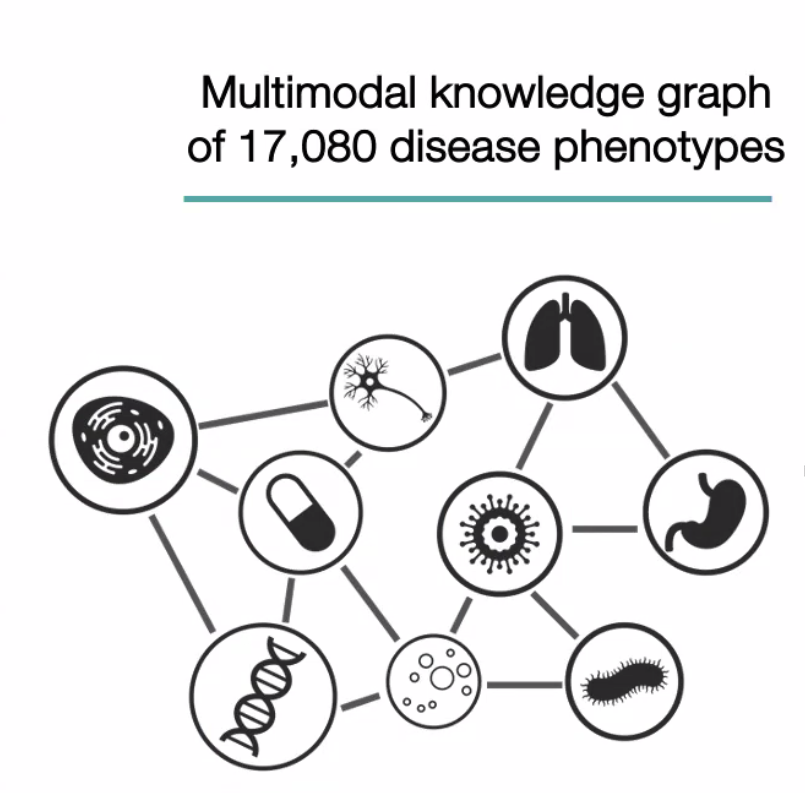
\includegraphics[scale=0.2]{MultimodalPreview.png}
    \end{figure}
    Image courtesy of partial figure from McDermott et al. {\it Structure-inducing pre-training} \cite{mcdermott_structure-inducing_2023}
\end{frame}


\begin{frame}{Molecular/Biochemical}
    \begin{figure}
        \centering
        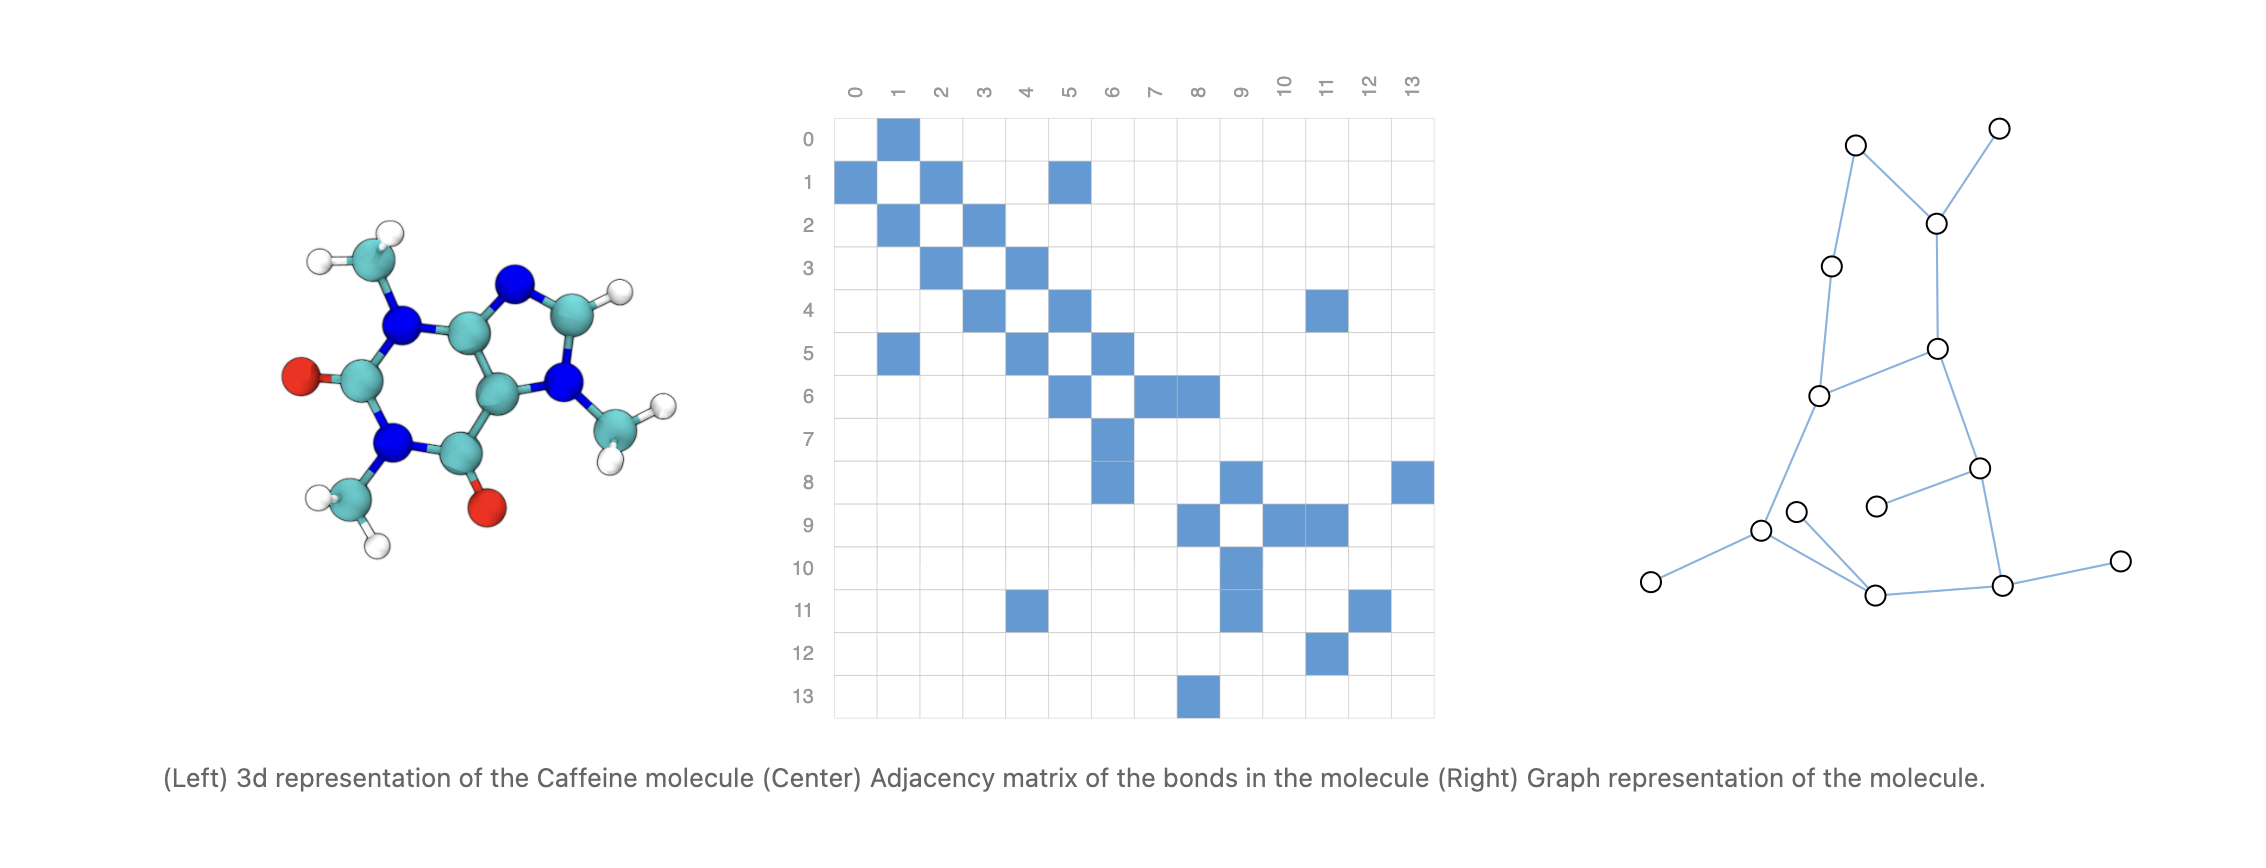
\includegraphics[scale=0.3]{Caffeine_Graph.png}
    \end{figure}
    Image courtesy of \url{https://distill.pub/2021/gnn-intro/} \cite{sanchez-lengeling_gentle_2021}
\end{frame}

\begin{frame}{Protein Folding \textcolor{red}{Maybe drop? 4 examples probably unnecessary}}
    \textcolor{red}{AlphaFold image/example here if I can find a nice one }
\end{frame}

\begin{frame}{Motivation}
    \begin{itemize}
        \item Want to utilize the input structure of the graph
        \begin{itemize}
            \item Respect/Maintain
            \item Update/Estimate
        \end{itemize} 
        \item "Flattening" graphical data for DNN, CNN, etc. omits useful topology from our data 
        \item Early methods attempting to retain topological info included recursive neural networks and random walk models, which GNN methodology extended \cite{scarselli_graph_2009} 
    \end{itemize}
\end{frame}



\begin{frame}{Notation/Set-Up}
    \begin{columns}[T] % align columns at the top
        \begin{column}{.7\textwidth}
            \begin{itemize}%{.5\textwidth}
                \setlength\itemsep{8mm}
%                \item Consider random vector $X \sim F(\boldsymbol\mu, \Sigma)$ and precision matrix $\Theta \equiv \Sigma^{-1}$
                \item Consider the graph $\Graph = (\NodeSet, \EdgeSet), \EdgeSet \subseteq \NodeSet \times \NodeSet$, where any node $\node$ has a related "feature vector" $x_\node \in \mathbb{R}^d$
                \begin{itemize}
                    \item Let $\NumNodes = \NumNodes$
                \end{itemize}
                \item Let $\nhood_s(\node)$ represent the $s$-hop neighborhood of any node $\node$ (and implicitly $\nhood(\node) \equiv \nhood_1(\node)$)
                \item Can construct adjacency matrix $\AdjMat \in \mathbb{R}^{\NumNodes \times \NumNodes}$ to capture structure of edge set $\EdgeSet$ 
                \begin{itemize} 
                    \item $\AdjMat_{ij}=w_{ij}\Ind\{(i,j) \in \EdgeSet\}$ for scalar weight $w_{ij} \in \mathbb{R}$
                \end{itemize}
            \end{itemize}
        \end{column}
        \begin{column}{.3\textwidth}
            %\begin{figure}
                \centering
            \scalebox{0.9}{
                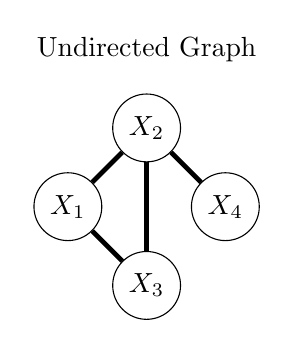
\begin{tikzpicture}
                \node[circle, draw] (A) at (0,0) {$X_1$};
                \node[circle, draw] (B) at (1,1) {$X_2$};
                \node[circle, draw] (C) at (1,-1) {$X_3$};
                \node[circle, draw] (D) at (2,0) {$X_4$};
                \node[] (capt) at (1, 2) {Undirected Graph};
                \draw[line width=0.6mm] (A) -- (B);
                \draw[line width=0.6mm] (A) -- (C);
                \draw[line width=0.6mm] (B) -- (D);
                \draw[line width=0.6mm] (C) -- (B);
            \end{tikzpicture}
            }
            %\caption{Undirected Graph}
            %\end{figure}
            \\ \vspace{3mm}
            \scalebox{0.9}{
            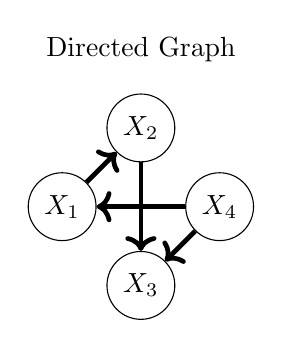
\begin{tikzpicture}%[opacity=0.2]
                \node[circle, draw] (A) at (0,0) {$X_1$};
                \node[circle, draw] (B) at (1,1) {$X_2$};
                \node[circle, draw] (C) at (1,-1) {$X_3$};
                \node[circle, draw] (D) at (2,0) {$X_4$};
                \node[] (capt) at (1, 2) {Directed Graph};
                \draw [line width=0.6mm, ->]
                    (A) edge (B)
                    (D) edge (A) 
                    (D) edge (C) 
                    (B) edge (C);
            \end{tikzpicture}
            }
        \end{column}
    \end{columns}
\end{frame}


\begin{frame}{Topology Representations}
\begin{itemize}\setlength
    \item Simplest/Na\"ive method is to use $\AdjMat$
    \item Consider also the Laplacian matrix $\LapMat = \DegMat - \AdjMat$ 
    \begin{itemize}
        \item $\mathbf{\DegMat = \text{diag}(A1_\NumNodes)}$
    \end{itemize}
    \item Can use an eigenvalue-normalized Laplacian $\LapMatNorm = \Identity - \DegMat^{-1/2}\AdjMat\DegMat^{-1/2} = \DegMat^{-1/2}\LapMat\DegMat^{-1/2}$
    \color{red}
    \item Define graph convolution here? 
    \item Note on necessity of permutation invariant functions (permutations of adjacency matrix represent same graph but consistent behavior of NN/GNN is not assured by permutd A matrices)
    \item Adjacency matrix can be prohibitively large but likely sparse, is also permutable but DNN's are not permutation invariant, undesirable 
    \item Can store an adjacency list
    \end{itemize}
\end{frame}



\section{General Construction \textcolor{red}{10-20ish minutes}}
\OutlineRedux 





\begin{frame}{What do we estimate about graph structure?}
    \textcolor{red}{See supp note 1 on Multimodal learning with graphs}
    \begin{gather*}
        \text{GNN learning can be }
        \begin{cases}
            \text{Node-wise }\Phi(\Graph, \node): (\node \in \NodeSet) \rightarrow \mathbb{R}^m 
            \\  \\ 
            \text{Edge-wise }\Phi(\Graph, \edge): (e\in \EdgeSet) \rightarrow \mathbb{R}^m  
            % can predict edge weights and prune to determine "edge presence", but I believe that GNN's take edge sets as input and preserve these edgesets 
            \\ \\ 
            \text{Graph-level characteristics }\Phi(\Graph) %\rightarrow \mathbb{R}^m 
            \end{cases}            
    \end{gather*}
\end{frame}


\begin{frame}{What do we estimate about graph structure?}
    \textcolor{red}{Planning (very tentatively) to note that I focus of node-wise estimation as primary interest. My understanding (with still much to read/learn) is that edge/graph-level characteristics are then essentially secondary outputs of node-characteristics. i.e. we fit the GNN, predict node labels/values/embeddings, then fit separate models to predict edge-/graph-level information}

    \begin{gather*}
        \text{GNN learning can be }
        \begin{cases}
            \text{Node-wise }\Phi(\Graph, x): (x\in \NodeSet) \rightarrow \mathbb{R}^m 
            \\  \\
            \tikz[baseline]{\node[anchor=base,fill=white,inner sep=0pt,opacity=0.5] {$\text{Graph-level characteristics }\Phi(\Graph, e): (e\in\EdgeSet) \rightarrow \mathbb{R}^m$};}
            \\ \\
            \tikz[baseline]{\node[anchor=base,fill=white,inner sep=0pt,opacity=0.5] {$\text{Graph-level characteristics }\Phi(\Graph)$};} %\rightarrow \mathbb{R}^m 
        \end{cases}            
    \end{gather*}
\end{frame}


\iffalse 
                    \begin{frame}{}
                        An overly simple representation: \newline 
                        \begin{columns}[T]
                        \begin{column}{0.3\textwidth}
                            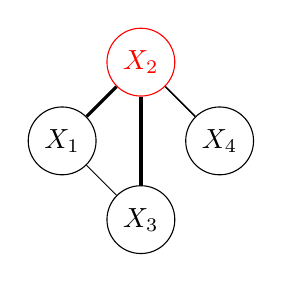
\begin{tikzpicture}
                                \node[circle, draw] (A) at (0,0) {$X_1$};
                                \node[circle, color=red, draw] (B) at (1,1) {$X_2$};
                                \node[circle, draw] (C) at (1,-1) {$X_3$};
                                \node[circle, draw] (D) at (2,0) {$X_4$};
                                \draw[line width=0.4mm] (A) -- (B);
                                \draw[line width=0.1mm] (A) -- (C);
                                \draw[line width=0.2mm] (B) -- (D);
                                \draw[line width=0.6mm] (C) -- (B);
                            \end{tikzpicture}
                        \end{column}
                        \begin{column}{0.4\textwidth}
                        % \begin{gather*}
                                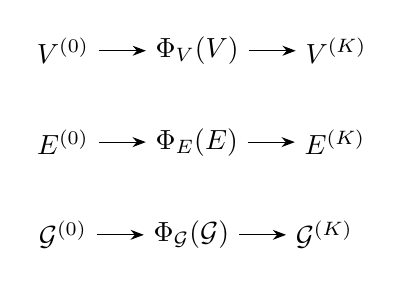
\begin{tikzpicture}[node distance=0.6cm,>=Stealth]
                                    % Nodes
                                    \node (NodeSet0) {$\NodeSet^{(0)}$};
                                    \node[right=of NodeSet0] (PhiNodeSet) {$\Phi_\NodeSet(\NodeSet)$};
                                    \node[right=of PhiNodeSet] (NodeSetIter) {$\NodeSet^{(\Iter)}$};
                                
                                    \node[below=of NodeSet0] (EdgeSet0) {$\EdgeSet^{(0)}$};
                                    \node[right=of EdgeSet0] (PhiEdgeSet) {$\Phi_\EdgeSet(\EdgeSet)$};
                                    \node[right=of PhiEdgeSet] (EdgeSetIter) {$\EdgeSet^{(\Iter)}$};
                                
                                    \node[below=of EdgeSet0] (Graph0) {$\Graph^{(0)}$};
                                    \node[right=of Graph0] (PhiGraph) {$\Phi_\Graph(\Graph)$};
                                    \node[right=of PhiGraph] (GraphIter) {$\Graph^{(\Iter)}$};
                                
                                    % Arrows
                                    \draw[->] (NodeSet0) -- (PhiNodeSet);
                                    \draw[->] (PhiNodeSet) -- (NodeSetIter);
                                
                                    \draw[->] (EdgeSet0) -- (PhiEdgeSet);
                                    \draw[->] (PhiEdgeSet) -- (EdgeSetIter);
                                
                                    \draw[->] (Graph0) -- (PhiGraph);
                                    \draw[->] (PhiGraph) -- (GraphIter);
                                \end{tikzpicture}
                        %\end{gather*}
                        \end{column}
                        \begin{column}{0.3\textwidth}
                            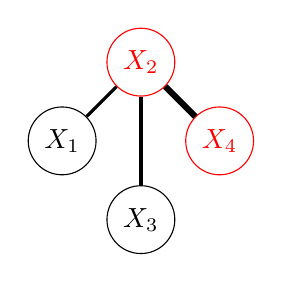
\begin{tikzpicture}
                                \node[circle, draw] (A) at (0,0) {$X_1$};
                                \node[circle, color=red, draw] (B) at (1,1) {$X_2$};
                                \node[circle, draw] (C) at (1,-1) {$X_3$};
                                \node[circle, color=red, draw] (D) at (2,0) {$X_4$};
                                \draw[line width=0.4mm] (A) -- (B);
                                %\draw[line width=0.1mm] (A) -- (C);
                                \draw[line width=0.8mm] (B) -- (D);
                                \draw[line width=0.5mm] (C) -- (B);
                            \end{tikzpicture}
                        \end{column}
                        \end{columns}

                    \end{frame}

\fi


\begin{frame}{
    General Framework\footnote{See \cite{ektefaie_multimodal_2023,gilmer_neural_2017, xu_how_2019}}
    }
    \textcolor{red}{Title NodeUpdate and create second slide with more clear backpropagation training (i.e. iter over NodeUpdate)} \newline
    General structure: 
    
    \begin{algorithmic}[1]
    \State Initialize $\nrepresent^{(0)} \gets x_\node, \forall \node \in \NodeSet$ 
        \For{$\iter = 0, ..., \Iter$}:
            \For{$\node \in \Graph$}:
            \State $\nrepresent_{agg}^{\iter+1} \gets \text{\textcolor{blue}{Aggregate}}(\{h_u^{(\iter)} \mid u \in \nhood_\node\})$ \qquad{\text{or \textcolor{blue}{Message$(\cdot)$}}}
            \State $\nrepresent^{(\iter+1)} \gets \text{\textcolor{blue}{Update}}(\nrepresent^{(\iter)}, \nrepresent_{agg}^{(\iter)})$
            \EndFor
        \EndFor
        \State $h_\Graph \gets \text{\textcolor{blue}{Transform}}(\{h^\Iter_\node | \node \in \Graph\})$ 
        \qquad{\hspace{4mm} or \textcolor{blue}{Readout$(\cdot)$}}
    \end{algorithmic}   

\end{frame}




\begin{frame}{General Framework}
Can succinctly represent the $\iter$th layer as: 
\begin{gather*}
    \mathbf{h}_\node^{(\iter+1)} 
    =
    \text{Update}
    \left( 
    x_\node^{(\iter)}
    ,   
    \text{Aggregate}
    (
        h_\node^{(\iter)}, x_u^{(\iter)}, \edge_{u,\node}^{(\iter)}
    )
    \right)
\end{gather*}

Choices of (differentiable) functions for Aggregate, Update, and Readout determine the architecture of your GNN 

\vspace{4mm}

Trained end-to-end via backpropagation

\end{frame}

\begin{frame}{Aggregate \& Update}
    \begin{itemize}
        \item {\bf Aggregate$(\cdot)$} produces a represntation of information from a node's neighborhood 
        \begin{itemize}
            \item Also {\bf Message$(\cdot)$} in the context of Message Passing Neural Networks (MPNN's) \cite{gilmer_neural_2017}
        \end{itemize}
        \item Differentiable, {\it permutation invariant} functions 
        \item Can include weights (edge-wise or learned)
        \item Over later iterations, this includes information from further and further distant nodes to any one target node 
    \end{itemize}

    \vspace{4mm}

    \begin{itemize}
        \item We then {\bf Update$(\cdot)$} our current state using this aggregated neighborhood-level information
    \end{itemize}
\end{frame}


\begin{frame}{Transform/Readout}
    \begin{itemize}
        \item {\bf Transform$(\cdot)$ } translates our learned node representations to some desired outcome 
        \begin{itemize}
            \item Regression
            \item Binary/Multi-class classification 
            \item MLP/DNN's 
        \end{itemize}
        \item {\bf Readout$(\cdot)$} is common term for translating node-level output to graph-level
        \begin{itemize}
            \item {\it Global Pooling} - Methods applied over entire graph (e.g. averaging, fitting "regular" deep neural network, etc.)
        \end{itemize}
    \end{itemize}
\end{frame}


\begin{frame}{Message Passing}
    \begin{itemize}
        \item Our {\bf Aggregate$(\cdot)$} step can also be thought 
    \end{itemize}
\end{frame}

\begin{frame}{Graph Convolutional Network}
\begin{align*}
    \NodeRepMat^{(\iter+1)}
    &=
    \sigma
    \left( 
        \AdjMat \NodeRepMat^{(\iter)} \Theta
    \right) 
\\
    \NodeRepMat^{(\iter+1)}
    &=
    \sigma
    \left( 
        \DegMat^{-1}\AdjMat \NodeRepMat^{(\iter)} \Theta
    \right) 
    \qquad{\text{Normalizing by degree for stability}}
\\
    \NodeRepMat^{(\iter+1)}
    &=
    \sigma
    \left( 
        \DegMat^{-1/2}\AdjMat\DegMat^{-1/2} \NodeRepMat^{(\iter)} \Theta
    \right) 
    \qquad{\text{Symmetric normalization}} % "no longer simple averaging"
\\
    \NodeRepMat^{(\iter+1)}
    &=
    \sigma
    \left( 
        \widetilde{\DegMat}^{-1/2}
        \widetilde{\AdjMat}
        \widetilde{\DegMat}^{-1/2} \NodeRepMat^{(\iter)} \Theta
    \right) 
    \qquad{\text{Adding self-loop}}
\end{align*}

where $\widetilde{\AdjMat} = \AdjMat + \Identity, \widetilde{\DegMat}_{ii} = \sum_j \widetilde{\AdjMat}_{ij}$, $\sigma$ is any activation function, $\NodeRepMat$ is simply the matrix of $\mathbf{\nrepresent}_\node$ for all nodes 
\end{frame}


\begin{frame}{Graph Convolutional Network}
    Proposed in 2017 by Thomas Kipf, Max Welling \cite{kipf_semi-supervised_2017}
        \begin{align*}
        \iffalse
            \mathbf{\nrepresent}_\node^{(\iter+1)} 
            &=
            \text{Update}
            \left( 
            x_\node^{(\iter)}
            ,   
            \text{Aggregate}
            (
                \nrepresent_\node^{(\iter)}, x_u^{(\iter)}, \edge_{u,\node}^{(\iter)}
            )
            \right)
        \\
        \fi 
            \NodeRepMat^{(\iter+1)} 
            &=
            \ReLu
            \left( 
                \mathbf{
                %D^{-1/2}
                %(\AdjMat + I)
                %D^{-1/2}
                \widetilde{\DegMat}^{-1/2}
                \widetilde{\AdjMat}
                \widetilde{\DegMat}^{-1/2}  
                \NodeRepMat^{(\iter)}
                \Theta 
                }            
            \right)
    \end{align*}
    
    \begin{itemize}
        %\item $\sigma(\cdot) = \text{ReLu}(\cdot)$ activation function
        \item Can replace ReLu with any activation function (e.g. sigmoid, GELU, etc.)
        \item Learned weight/parameter matrix $\boldsymbol\Theta$
        %\item $\mathbf{D}_{ii} = \sum_{j}\mathbf{(\AdjMat+I)_{ij}}$
        %\item Eigenvalue normalizing $\mathbf{D^{-1/2}(\AdjMat + I)D^{-1/2}}$ for computational stability
    \end{itemize}
    \textcolor{red}{Review paper, comment on applications briefly (KG setting), also motivate through graph convolutions?}
    \end{frame}

\begin{frame}{Graph Convolutional Network}
    Proposed in 2017 by Thomas Kipf, Max Welling \cite{kipf_semi-supervised_2017}
        \begin{align*}
        \iffalse
            \mathbf{\nrepresent}_\node^{(\iter+1)} 
            &=
            \text{Update}
            \left( 
            x_\node^{(\iter)}
            ,   
            \text{Aggregate}
            (
                \nrepresent_\node^{(\iter)}, x_u^{(\iter)}, \edge_{u,\node}^{(\iter)}
            )
            \right)
        \\
        \fi 
            \NodeRepMat^{(\iter+1)} 
            &=
            \underbrace{\ReLu}_{\text{Update}}
            \underbrace{
            \left( 
                \mathbf{
                %D^{-1/2}
                %(\AdjMat + I)
                %D^{-1/2}
                \widetilde{\DegMat}^{-1/2}
                \widetilde{\AdjMat}
                \widetilde{\DegMat}^{-1/2}  
                \NodeRepMat^{(\iter)}
                \Theta 
                }            
            \right)
            }_{\text{Aggregate/Message}}
    \end{align*}
    
    \begin{itemize}
        %\item $\sigma(\cdot) = \text{ReLu}(\cdot)$ activation function
        \item Can replace ReLu with any activation function (e.g. sigmoid, GELU, etc.)
        \item Learned weight/parameter matrix $\boldsymbol\Theta$
        %\item $\mathbf{D}_{ii} = \sum_{j}\mathbf{(\AdjMat+I)_{ij}}$
        %\item Eigenvalue normalizing $\mathbf{D^{-1/2}(\AdjMat + I)D^{-1/2}}$ for computational stability
    \end{itemize}
    \textcolor{red}{Review paper, comment on applications briefly (KG setting), also motivate through graph convolutions?}
    \end{frame}



\section{Applications and Extensions \textcolor{red}{20-25ish minutes}}
\OutlineRedux


\subsection{Knowledge-Graph Data}

\subsection{Multimodal Biomedical Data}

\begin{frame}{Motivation}
\end{frame}



\begin{frame}{}
    \bf{\LARGE Conclusion}    
\end{frame}

\section*{Conclusion}



\begin{frame}[allowframebreaks]{References}
    \begin{itemize}
    \item Some diagrams generated in conjunction with ChatGPT 3.5
    \end{itemize}
    \printbibliography 
\end{frame}


%%%%%%%%%%%%%%%%%%%%%%%%%%
%%%%%%%%%%%%%%%%%%%%%%%%%%
% Appendix 
%%%%%%%%%%%%%%%%%%%%%%%%%%
%%%%%%%%%%%%%%%%%%%%%%%%%%

\section*{Appendix}

\begin{frame}{}
\bf{\LARGE Appendix Slides}    
\end{frame}

\begin{frame}{Implementations}
    \begin{itemize}
        \item \href{https://pytorch-geometric.readthedocs.io/en/latest/}{PyTorch Geometric} with directed extension \href{https://github.com/SherylHYX/pytorch_geometric_signed_directed}{PyTorch Geometric Signed Directed}
        \item \href{https://github.com/tensorflow/gnn}{TensorFlow GNN} \cite{ferludin_tf-gnn_2023}
        \item \href{https://carlolucibello.github.io/GraphNeuralNetworks.jl/dev/}{GraphNeuralNetworks.jl}
        \item \href{https://graphneural.network/}{Spektral}, Keras-based Pythhon package 
        \item Limited but some implementation in R 
        \begin{itemize}
            \item \href{https://cran.r-project.org/web/packages/scapGNN/vignettes/vignette.html}{scapGNN}, package GNN implementation but specific/narrow for single-cell -omics data 
        \end{itemize}
    \end{itemize}
\end{frame}

\begin{frame}{Abbreviated History}
    \begin{itemize}
        \item Graph Neural Network first(?) coined in Gori (2005) \cite{gori_new_2005} and subqeuently in Scarselli (2009) {\it The Graph Neural Network Model} \cite{scarselli_graph_2009}
        \item Graph Convolutional Network by Kipf (2017) \cite{kipf_semi-supervised_2017} but with similar convolutional message-passing algorithms (within GNN's) proposed in at least 2015 \cite{duvenaud_convolutional_2015}
        \item Message passing GNN proposed in Gilmer (2017), applications in molecular chemistry \cite{gilmer_neural_2017} 
    \end{itemize}
\end{frame}

\begin{frame}[allowframebreaks]{Additional Applications, Interesting Papers}
    \begin{itemize}
        \item Applications in travel time prediction, 2021 (\url{https://arxiv.org/pdf/2108.11482.pdf})
        \item Someone has compiled graph-/GNN-relevant talks for NeurIPS 2023 at \url{https://github.com/XiaoxinHe/neurips2023_learning_on_graphs}
    \end{itemize}
\end{frame}

\begin{frame}{DiffPool}
    Figure 1 from Ying (2018) {\it Hierarchical Graph Representation Learning with Differentiable Pooling} \cite{ying_hierarchical_2018}
    \begin{figure}
        \centering 
        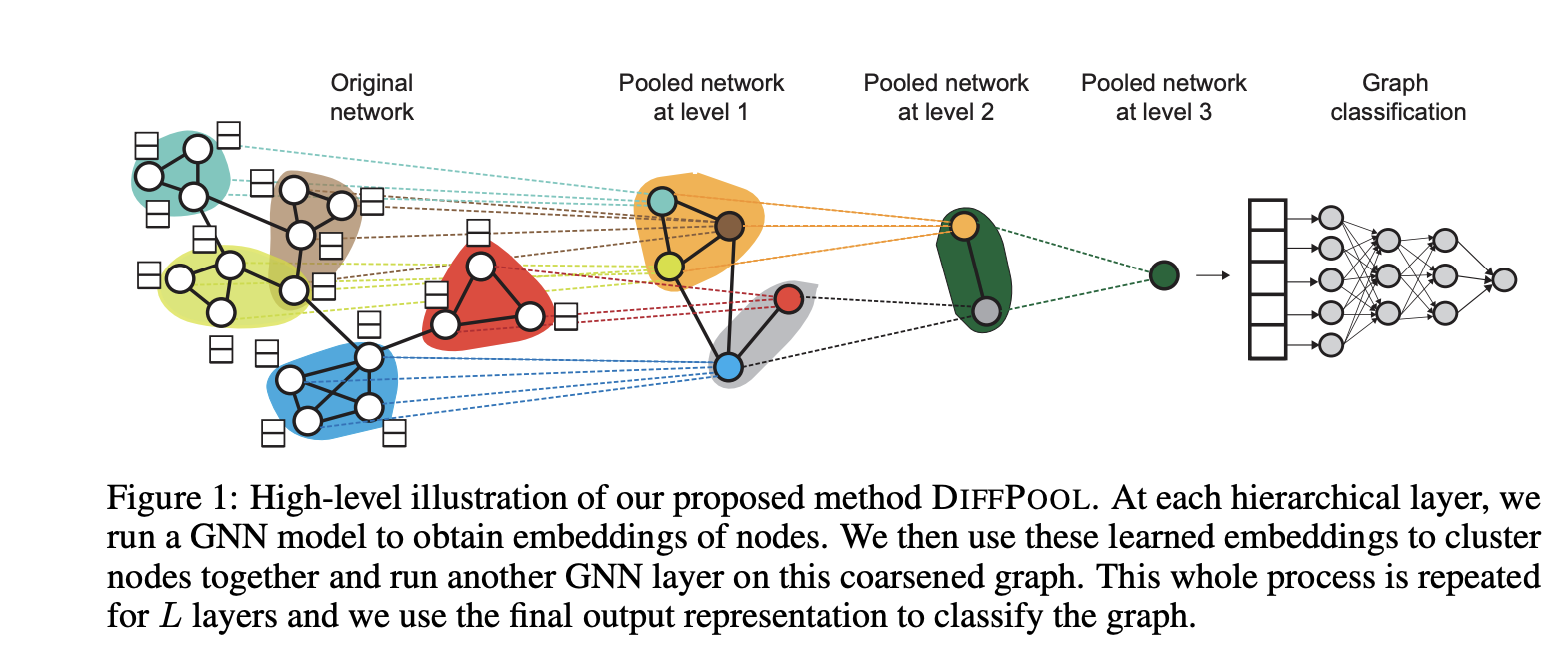
\includegraphics[scale=0.45]{DIFFPOOL_RexYing.png}
    \end{figure}
\end{frame}

\begin{frame}{KG AI Models}
    Full figure from McDermott et al. \cite{mcdermott_structure-inducing_2023}, cropped and presented in Introduction:
    \begin{figure}
        \centering
        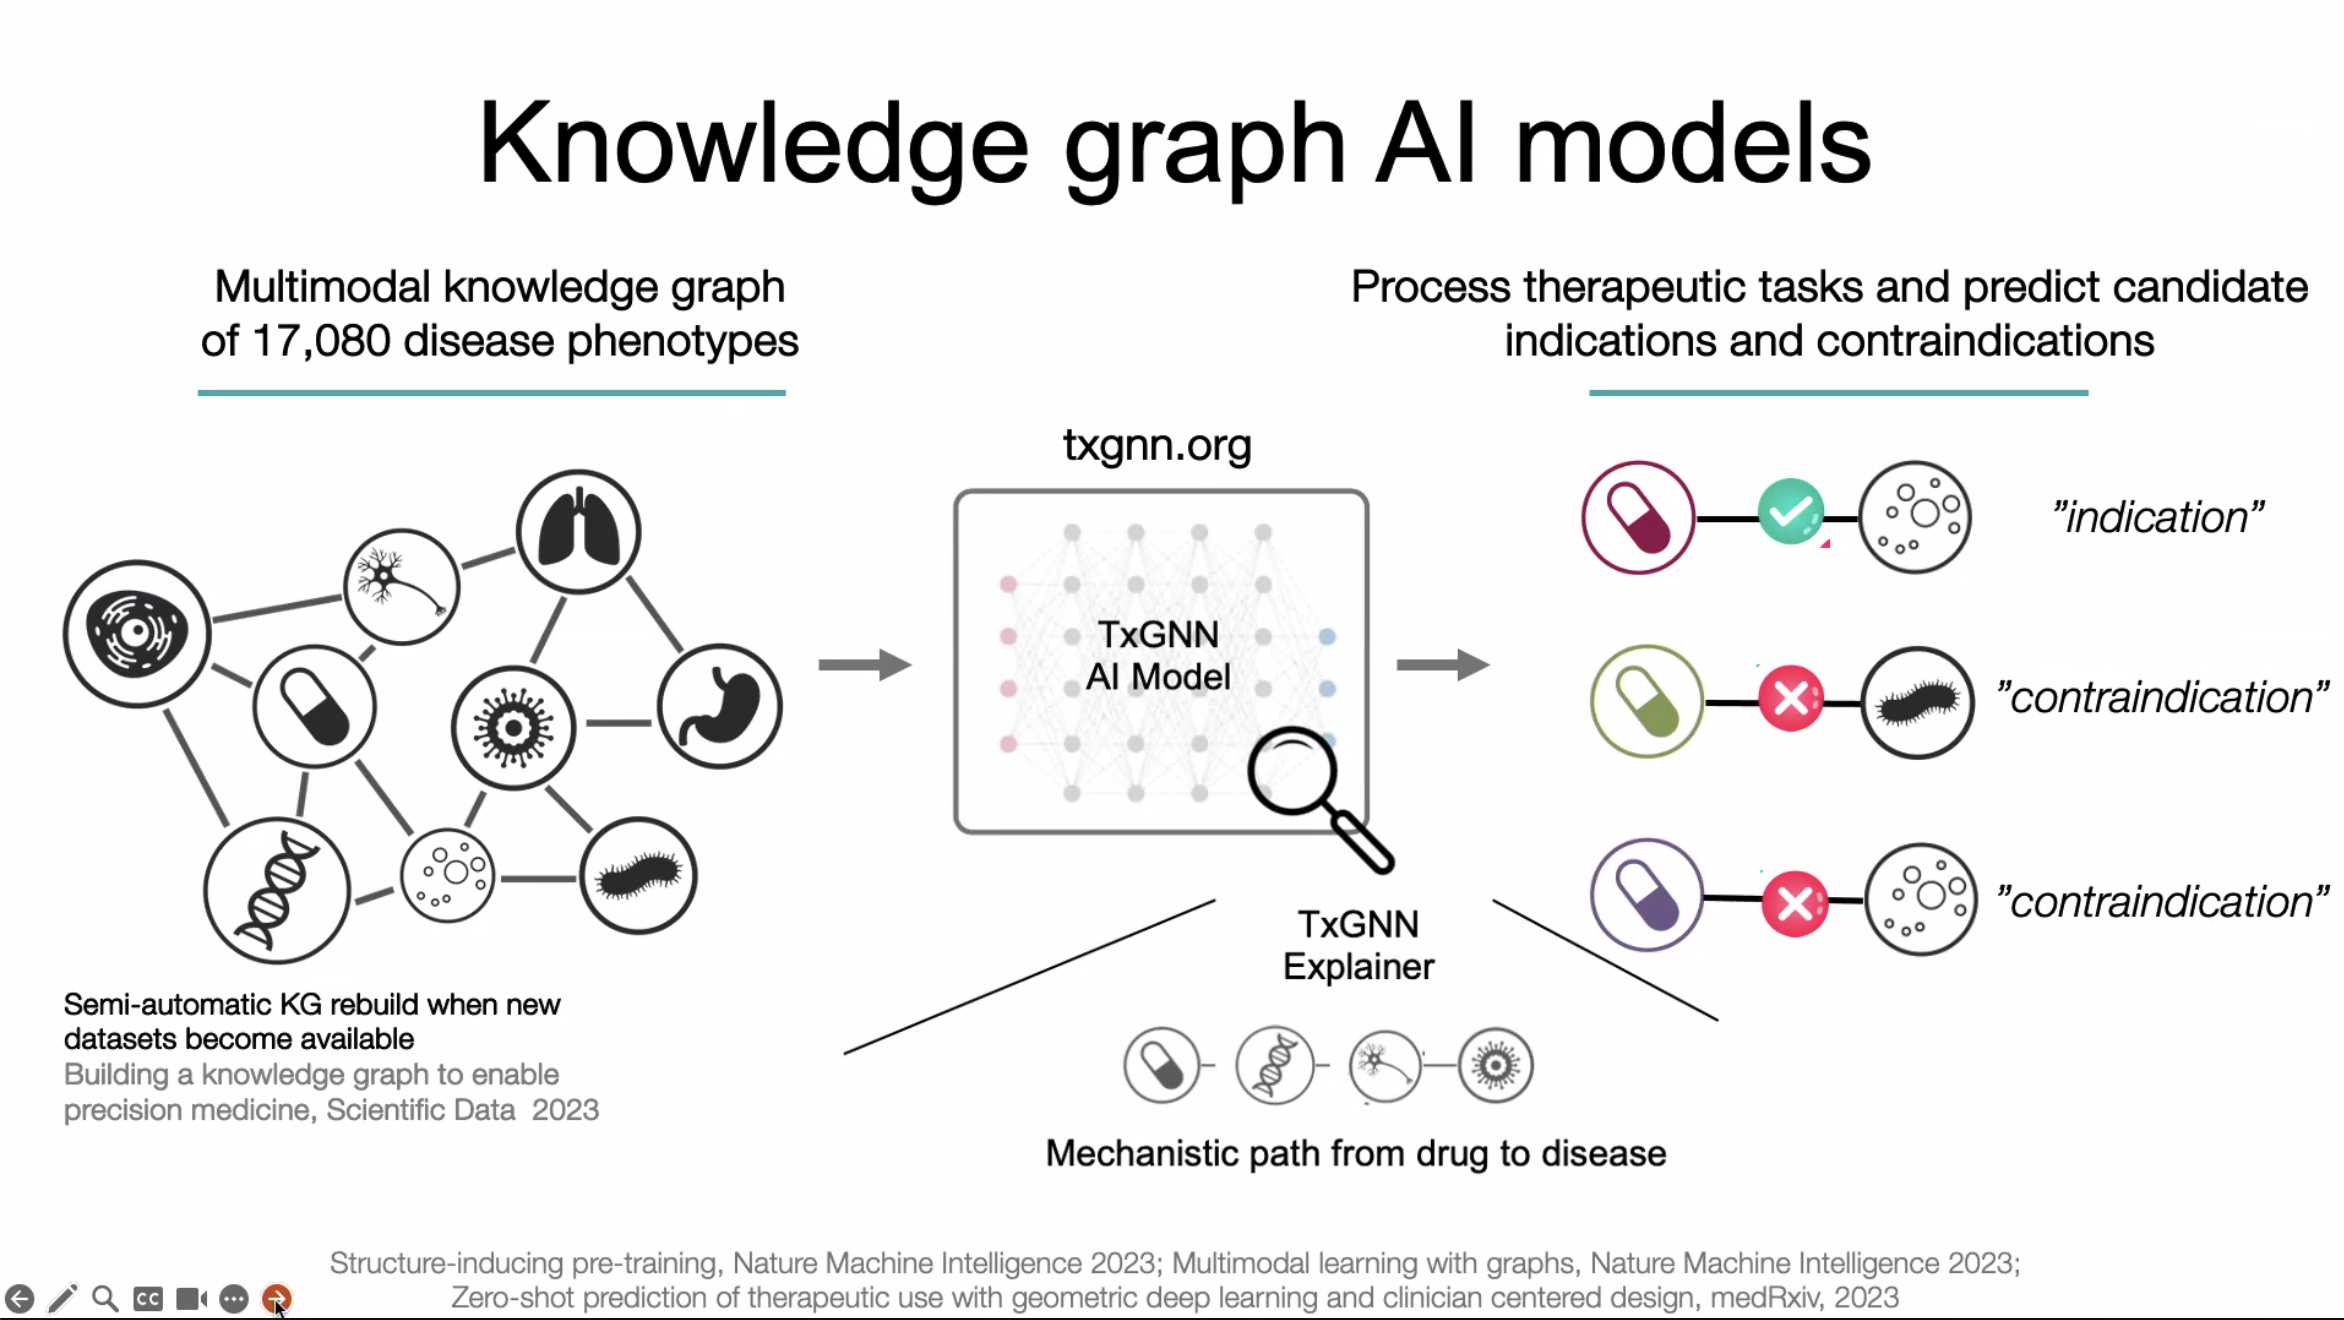
\includegraphics[scale=0.13]{Junwei_KG_Models_Infograph.png}
    \end{figure}
\end{frame}
\end{document}